\section{Target File Generator} \label{target_generator}

Once the software is ready, it must be tested on several target files, first to be sure it's working properly, and then to work on the convergence rate's improvement. For this purpose, a program called "target_generator" has been created. It is able to create five types of target distribution : Random, Random with a normal distribution, Focused, Focused with a normal distribution, and Homogeneous. An example of each one of those is available on Figure \ref{fig:target_generator:examples}.
\\

\begin{figure}[h]
	\begin{center}
		\begin{subfigure}{0.32\textwidth}
			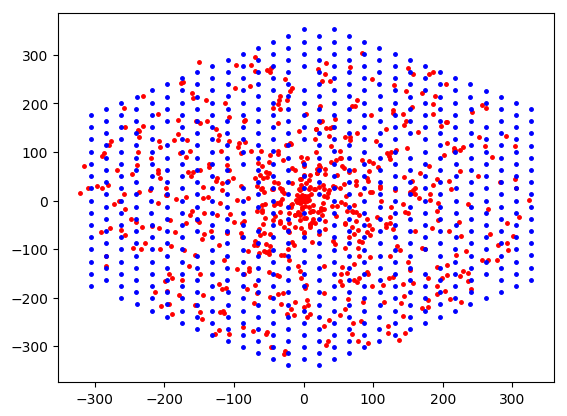
\includegraphics[width=\textwidth]{target/random.png}
			\caption{Example of target file with a random distribution.}
		\end{subfigure}
		\begin{subfigure}{0.32\textwidth}
			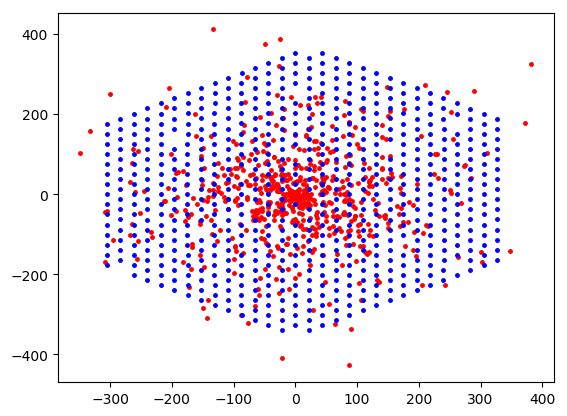
\includegraphics[width=\textwidth]{target/random_normal.png}
			\caption{Example of target file with a random and normal distribution.}
		\end{subfigure}
		\begin{subfigure}{0.32\textwidth}
			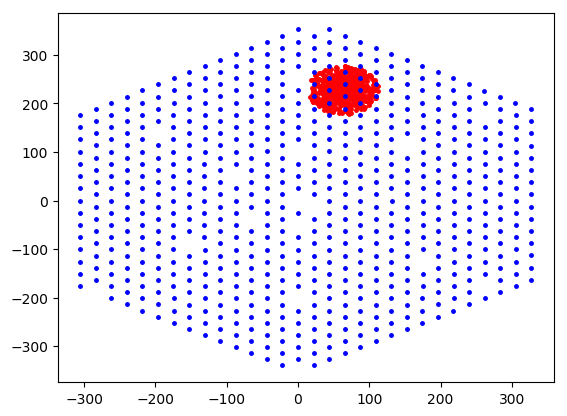
\includegraphics[width=\textwidth]{target/focus.png}
			\caption{Example of target file with a distribution focused on a random point of the telescope.}
		\end{subfigure}
		
		\begin{subfigure}{0.32\textwidth}
			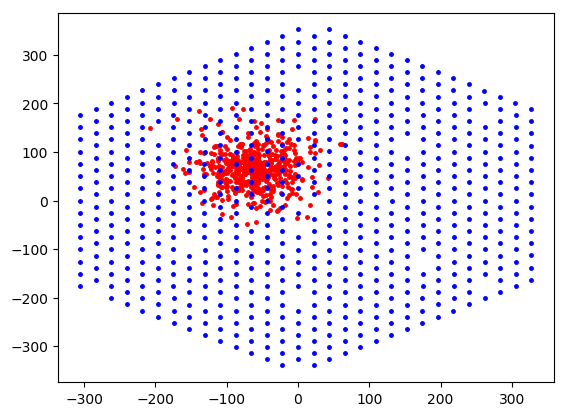
\includegraphics[width=\textwidth]{target/focus_normal.png}
			\caption{Example of target file with a normal distribution focused on a random point of the telescope.}
		\end{subfigure}
		\begin{subfigure}{0.32\textwidth}
			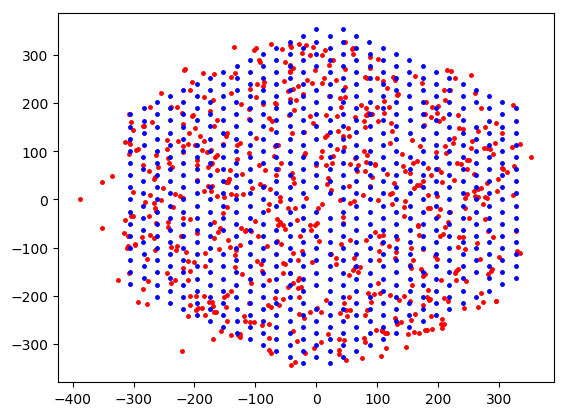
\includegraphics[width=\textwidth]{target/homogeneous.png}
			\caption{Example of target file with an homogeneous distribution.}
		\end{subfigure}
		\caption{Examples of target files generated with the target_generator.py program. Targets are shown in red, while actuators are shown in blue. Actuator positions come from the former software (used for MOONS), and therefore contains its specificity, that is to say some holes where fiducial tools were positioned.}
		\label{fig:target_generator:examples}
	\end{center}
\end{figure}

The homogeneous is the most similar to the MOONS's target files, as it places a target close to each actuators. Therefore, it will also be the one with the highest convergence rate.